% set documentclass - this will make the file compile if open in editor
\documentclass[a4paper,12pt,fullpage,openany,hyperfootnotes,hidelinks]{scrbook}

% load Tikz & related packages
\usepackage{tikz}
\usetikzlibrary{matrix,arrows.meta,fit,positioning,shapes,automata}
\usepackage{forest}

% document must begin
\begin{document}

% notes on graphics goal / textual description of what is to be conveyed
% INSERT

% existing sketch of the graphics
% INSERT
%\begin{figure}[htp]
%    \centering
%    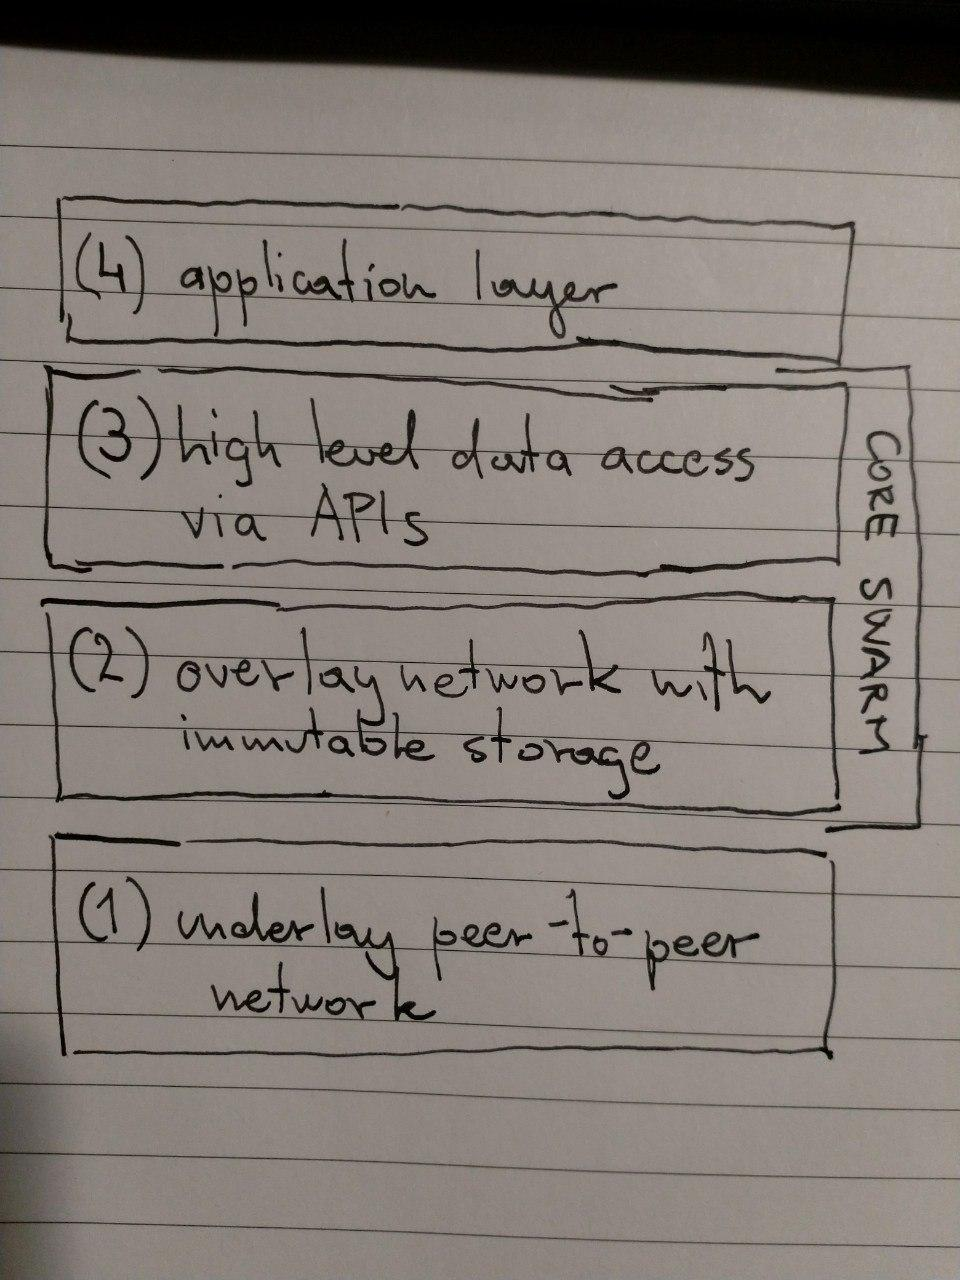
\includegraphics[width=10cm]{fig-drafts/swarm-layered-design.jpg}
%\end{figure}

% simple example Tikz "picture"
% \begin{figure}[htbp]
% \centering
% \resizebox{1\textwidth}{!}{
%     \begin{tikzpicture}[
level/.style={sibling distance=15mm, line width=0.6pt, level distance=18mm},
hash/.style={fill=white, rounded corners=2pt,draw,minimum size=1.2cm},
chunk/.style={fill=lightgray, rounded corners=2pt,draw,minimum size=1.2cm},
midchunk/.style={fill=lightgray!50, rounded corners=2pt,draw,minimum size=1.2cm}
]

% root node
\node [hash] (root) {$H$}
  % vertical arrow
  child[grow=down,draw=none] { node {} edge from parent[<-,shorten >=12pt]}
  % annotation
  child[grow=right,draw=none,level distance=5cm] { node (swh) {Swarm root hash} edge from parent[draw=none] }
  % level n-1
  child {node [hash] (n-10) {$H_{0}$} edge from parent[draw=none]
    % arrow
    child[grow=down,draw=none] { node {} edge from parent[<-, shorten >=12pt]}
    % annotation
    child[grow=left,draw=none,level distance=4cm] { node[align=center] (bnl) {intermediate\\branching nodes\\chunks of 128 hashes}  edge from parent[draw=none] }
    % level n-2
    child {node [hash] (n-2l0) {$H_{0}$} edge from parent[draw=none]
      % level 2
      child[thick] {node [midchunk] (2l0) {$C$} edge from parent[draw=none]
        % level 1
        child[grow=down,draw=none] { node {} edge from parent[<-, shorten >=18pt, ultra thick]}
        child {node [hash] (1l0) {$H_{0}$} edge from parent[draw=none]
          % level 0
          child[grow=down,draw=none] { node {} edge from parent[<-, shorten >=12pt]}
          child {node [hash] (0l0) {$H_{0}$} edge from parent[<-, draw=none]
            child {node [chunk] {$C_{0}$}}
          }
          child {node [hash] (0l1) {$H_{1}$} edge from parent[<-, draw=none]
            child {node [chunk] (cl1) {$C_{1}$}}
          }
          child[missing]
          child {node [hash] (0ll) {$H_{127}$} edge from parent[<-, draw=none]
            child {node [chunk] (cll) {$C_{i}$}}
          }
        }
        % level 1 siblings
        child {node [hash] (1l1) {$H_{1}$} edge from parent[draw=none]
          child[thick,loosely dotted, shorten >=6mm, thick,<-] {node {}}
        }
        child[missing]
        child {node [hash] (1ll) {$H_{127}$} edge from parent[draw=none]
          child[thick,loosely dotted, shorten >=6mm, thick,<-] {node {}}
        }
      }
    }
    % level n-2 siblings lhs
    child {node [hash] (n-2l1) {$H_{1}$} edge from parent[draw=none]
      child[thick,loosely dotted, shorten >=6mm, thick,<-] {node {}}
    }
    child[missing]
    child {node [hash] (n-2ll) {$H_{127}$} edge from parent[draw=none]
      child[thick,loosely dotted, shorten >=6mm, thick,<-] {node {}}
    }
  }
  % level n-1 siblings
  child {node [hash] (n-11) {$H_{1}$} edge from parent[draw=none]
    child[thick,loosely dotted, shorten >=6mm, thick,<-] {node {}}
  }
  child[missing]
  child[missing]
  child[missing]
  child {node [hash] (n-1l) {$H_{127}$} edge from parent[draw=none]
    % level n-2 siblings rhs vertical arrow
    child[grow=down,draw=none] { node {} edge from parent[<-, shorten >=12pt]}
    child[grow=right,level distance=9cm] { node[align=center] (bnr)  {intermediate\\branching nodes\\chunks of 128 hashes} edge from parent[draw=none]}
    child[missing]
    child {node [hash] (n-2r0) {$H_{0}$} edge from parent[draw=none]
      child[thick,loosely dotted, shorten >=6mm, thick,<-] {node {}}
    }
    child[missing]
    child {node [hash] (n-2r1) {$H_{i}$} edge from parent[draw=none]
      child[thick,loosely dotted, shorten >=6mm, thick,<-] {node {}}
    }
    child[missing]
    child {node [hash] (n-2rl) {$H_{127}$} edge from parent[draw=none]
      % level 2 siblings
      child[grow=down] {node [midchunk] (2rl) {$C$} edge from parent[draw=none]
        child[grow=down,draw=none] { node {} edge from parent[<-, shorten >=18pt, ultra thick]}
        child {node [hash] (1r0) {$H_{0}$} edge from parent[draw=none]
          child[thick,loosely dotted, shorten >=6mm, thick,<-] {node {}}
        }
        child[missing]
        child {node [hash] (1r1) {$H_{i}$} edge from parent[draw=none]
          child[thick,loosely dotted, shorten >=6mm, thick,<-] {node {}}
        }
        % child[missing]
        child[missing]
        child {node [hash] (1rl) {$H_{127}$} edge from parent[draw=none]
          child[grow=down,draw=none] { node {} edge from parent[<-, shorten >=12pt]}
          child {node [hash] (0r0) {$H^_{0}$} edge from parent[<-, draw=none]
            child {node [chunk] (cr0) {$C_{i}$}}
          }
          child {node [hash] (0r1) {$H^_{1}$} edge from parent[<-, draw=none]
            child {node [chunk] (cr1) {$C_{i}$}}
          }
          child[missing]
          child {node [hash] (0rl) {$H_{127}$} edge from parent[<-, draw=none]
            child {node [chunk] (crl) {$C_{m}$}
              child [grow=right] { edge from parent[draw=none]
                child [grow=right] {node[align=center] {leaf chunks\\data level} edge from parent[draw=none]
                  child [grow=up] {node {level $0$} edge from parent[draw=none]
                    child [grow=up] {node {level $1$} edge from parent[draw=none]
                      child [grow=up] {node (l2) {level $2$} edge from parent[draw=none]
                        child [grow=up] {node (ln-2) {level $n-2$} edge from parent[draw=none]
                          child [grow=up] {node {level $n-1$} edge from parent[draw=none]
                            child [grow=up] {node {root = level $n$} edge from parent[draw=none]}
                          }
                        }
                      }
                    }
                  }
                }
              }
            }
          }
        }
      }
    }
  };

% elipsis
\path (n-11) -- (n-1l) node [midway,font=\large] {$\ldots$};
\path (n-2l0) -- (2l0) node [midway,font=\large,sloped] {$\ldots$};
\path (n-2rl) -- (2rl) node [midway,font=\large,sloped] {$\ldots$};
\path (ln-2) -- (l2) node [midway,font=\large,sloped] {$\ldots$};
\path (1l1) -- (1ll) node [midway,font=\large] {$\ldots$};
\path (1r1) -- (1rl) node [midway,font=\large] {$\ldots$};
\path (1ll) -- (1r0) node [midway,font=\large] {$\ldots$};
\path (n-2l1) -- (n-2ll) node [midway,font=\large] {$\ldots$};
\path (n-2r1) -- (n-2rl) node [midway,font=\large] {$\ldots$};
\path (n-2ll) -- (n-2r0) node [midway,font=\large,sloped] {$\ldots$};
\path (0l1) -- (0ll) node [midway,font=\large] {$\ldots$};
\path (0r1) -- (0rl) node [midway,font=\large] {$\ldots$};
\path (0ll) -- (0r0) node [midway,font=\large] {$\ldots$};
\path (cl1) -- (cll) node [midway,font=\large] {$\ldots$};
\path (cr1) -- (crl) node [midway,font=\large] {$\ldots$};
\path (cll) -- (cr0) node [midway,font=\large] {$\ldots$};
\path (2l0) -- (2rl) node [midway,font=\large] {$\ldots$};
 

% arrows from annotations
\begin{scope}[shorten >=.5cm,thin]
\draw [->] (swh) -> (root);
\draw [->] (bnl) -> (n-10);
\draw [->] (bnl) -> (n-2l0);
\draw [->] (bnl) -> (1l0);
\draw [->] (bnl) -> (0l0);
\draw [->] (bnr) -> (n-1l);
\draw [->] (bnr) -> (n-2rl);
\draw [->] (bnr) -> (1rl);
\draw [->] (bnr) -> (0rl);
\end{scope}

% boxes to group nodes
\node[rounded corners=2pt, draw=white, minimum height=1.1cm, fit=(root)] {};
\node[rounded corners=2pt, draw=black, minimum height=1.1cm, fit=(0l0) (0ll)] {};
\node[rounded corners=2pt, draw=black, minimum height=1.1cm, fit=(n-2l0) (n-2ll)] {};
\node[rounded corners=2pt, draw=black, minimum height=1.1cm, fit=(n-2r0) (n-2rl)] {};
\node[rounded corners=2pt, draw=black, minimum height=1.1cm, fit=(1l0) (1ll)] {};
\node[rounded corners=2pt, draw=black, minimum height=1.1cm, fit=(1r0) (1rl)] {};
\node[rounded corners=2pt, draw=black, minimum height=1.1cm, fit=(n-10) (n-1l)] {};
\node[rounded corners=2pt, draw=black, minimum height=1.1cm, fit=(0r0) (0rl)] {};

\end{tikzpicture}
% }
% \caption[Swarm hash]{Swarm hash}
% \label{fig:Swarm-hash}
% \end{figure}

% \begin{figure}[htbp]
%     \centering
%     % not sure about these colours!
\definecolor{c1}{HTML}{FF7F00}
\definecolor{c2}{HTML}{048BA8}
\definecolor{c3}{HTML}{16DB93}
\definecolor{c4}{HTML}{EFEA5A}
\definecolor{c5}{HTML}{F29E4C}
\definecolor{c6}{HTML}{256EFF}
\definecolor{c7}{HTML}{46237A}

\scalebox{1.35}{
\begin{forest}
rt/.style={draw=blue,line width=1pt},
peer/.style={draw=blue!60,edge={blue!60,line width=0.7pt}},
peerleaf/.style={edge={blue!60,line width=0.7pt}},
self/.style={draw=blue,fill=blue,edge={blue,line width=1pt}},
selfpeer/.style={draw=blue,line width=1pt,edge={blue,line width=1pt}},
unused/.style={draw=blue!20,edge={blue!20,line width=0.7pt}},
[{},rt,for tree={circle,draw, l sep=20pt}
  [{},selfpeer,edge label={node[midway,left] {0}}
    [{},peer,edge label={node[midway,left] {0}}
      [{},peer,edge label={node[midway,left] {0}}
        [{},unused,edge label={node[midway,left] {0}}]
        [{},peerleaf,fill=c1,draw=c1,edge label={node[midway,right] {1}}]
      ]
      [{},peer,edge label={node[midway,right] {1}}
        [{},peerleaf,fill=c2,draw=c2,edge label={node[midway,left] {0}}]
        [{},unused,edge label={node[midway,right] {1}}]
      ]
    ]
    [{},selfpeer,edge label={node[midway,right] {1}} 
      [{},selfpeer,edge label={node[midway,left] {0}}
        [{},peerleaf,fill=c3,draw=c3,edge label={node[midway,left] {0}}]
        [{},self,edge label={node[midway,right] {1}}]
      ]
      [{},peer,edge label={node[midway,right] {1}}
        [{},peerleaf,fill=c4,draw=c4,edge label={node[midway,left] {0}}]
        [{},peerleaf,fill=c5,draw=c5,edge label={node[midway,right] {1}}]
      ]
    ] 
  ]
  [{},peer,edge label={node[midway,right] {1}}
    [{},unused,edge label={node[midway,left] {0}}
      [{},unused,edge label={node[midway,left] {0}}
        [{},unused,edge label={node[midway,left] {0}}]
        [{},unused,edge label={node[midway,right] {1}}]
      ]
      [{},unused,edge label={node[midway,right] {1}}
        [{},unused,edge label={node[midway,left] {0}}]
        [{},unused,edge label={node[midway,right] {1}}]
      ]
    ]
    [{},peer,edge label={node[midway,right] {1}} 
      [{},peer,edge label={node[midway,left] {0}}
        [{},fill=c6,peerleaf,draw=c6,edge label={node[midway,left] {0}}]
        [{},unused,edge label={node[midway,right] {1}}]
      ]
      [{},peer,edge label={node[midway,right] {1}}
        [{},fill=c7,peerleaf,draw=c7,edge label={node[midway,left] {0}}]
        [{},unused,edge label={node[midway,right] {1}}]
      ]
    ]
  ] 
]
\end{forest}
}
%     \caption[Forwarding Kademlia routing]{TBD Forwarding Kademlia routing}
%     \label{fig:forwarding-kademlia}
% \end{figure}

% \begin{figure}[htbp]
%     \centering
%     % not sure about these colours!
\definecolor{c1}{HTML}{FF7F00}
\definecolor{c2}{HTML}{048BA8}
\definecolor{c3}{HTML}{16DB93}
\definecolor{c4}{HTML}{EFEA5A}
\definecolor{c5}{HTML}{F29E4C}
\definecolor{c6}{HTML}{256EFF}
\definecolor{c7}{HTML}{46237A}

\scalebox{1.35}{
\begin{forest}
rt/.style={draw=blue,line width=1pt},
peer/.style={draw=blue!60,edge={blue!60,line width=0.7pt}},
peerleaf/.style={edge={blue!60,line width=0.7pt}},
self/.style={draw=blue,fill=blue,edge={blue,line width=1pt}},
selfpeer/.style={draw=blue,line width=1pt,edge={blue,line width=1pt}},
unused/.style={draw=blue!20,edge={blue!20,line width=0.7pt}},
[{},rt,for tree={circle,draw, l sep=20pt}
  [{},selfpeer,edge label={node[midway,left] {0}}
    [{},selfpeer,edge label={node[midway,left] {0}}
      [{},selfpeer,edge label={node[midway,left] {0}}
        [{},self,edge label={node[midway,left] {0}}]
        [{},draw=c3,fill=c3,peerleaf,edge label={node[midway,right] {1}}]
      ]
      [{},peer,edge label={node[midway,right] {1}}
        [{},draw=c4,fill=c5,peerleaf,edge label={node[midway,left] {0}}]
        [{},draw=c4,fill=c4,peerleaf,edge label={node[midway,right] {1}}]
      ]
    ]
    [{},peer,edge label={node[midway,right] {1}} 
      [{},peer,edge label={node[midway,left] {0}}
        [{},draw=c1,fill=c1,peerleaf,edge label={node[midway,left] {0}}]
        [{},unused,edge label={node[midway,right] {1}}]
      ]
      [{},peer,edge label={node[midway,right] {1}}
        [{},unused,edge label={node[midway,left] {0}}]
        [{},draw=c2,fill=c2,peerleaf,edge label={node[midway,right] {1}}]
      ]
    ] 
  ]
  [{},peer,edge label={node[midway,right] {1}}
    [{},peer,edge label={node[midway,left] {0}}
      [{},peer,edge label={node[midway,left] {0}}
        [{},unused,edge label={node[midway,left] {0}}]
        [{},draw=c6,fill=c6,peerleaf,edge label={node[midway,right] {1}}]
      ]
      [{},peer,edge label={node[midway,right] {1}}
        [{},unused,edge label={node[midway,left] {0}}]
        [{},draw=c7,fill=c7,peerleaf,edge label={node[midway,right] {1}}]
      ]
    ]
    [{},unused,edge label={node[midway,right] {1}} 
      [{},unused,edge label={node[midway,left] {0}}
        [{},unused,edge label={node[midway,left] {0}}]
        [{},unused,edge label={node[midway,right] {1}}]
      ]
      [{},unused,edge label={node[midway,right] {1}}
        [{},unused,edge label={node[midway,left] {0}}]
        [{},unused,edge label={node[midway,right] {1}}]
      ]
    ]
  ] 
]
\end{forest}
}
%     \caption[Forwarding Kademlia routing]{TBD Forwarding Kademlia routing}
%     \label{fig:forwarding-kademlia}
% \end{figure}

\begin{figure}[htbp]
   \centering
   \caption[Kademlia table (recursive flavour)]{\gloss{Kademlia table} (recursive flavour):  peers of node $x$ partitioned into proximity order bins. Saturated Kademlia connectivity is 
   characterised by a live Kademlia table of directly connected TCP peers such that (1) there is at least $k$ peers in each bin up to but excluding saturation depth $d_x$ and (2) all the nodes in the entire network that would fall in a bin higher or equal to $d_x$ are actually peers of $x$. }
   \caption[Forwarding Kademlia routing]{TBD Forwarding Kademlia routing}
   \label{fig:kademlia-table}
\end{figure}

% document must end
\end{document}